\chapter{Inledning}

Mängden av producerad data ökar helta tiden, och kräver därför kraftigare och pålitligare
metoder för att hantera datan. Ett exempel på helheter som skapar mycket data i form av
dataströmmar är \textit{sakernas internet} (Internet of Things, IoT) system som \textit{smarta städer}
(Smart Cities) var data samlas från sensorer och mobiltelefoner \citep{vakali2014smart}
eller i sjöfart var data samlas från skepp \citep{xu2019internet}. Utvinnande och analysering
av massiva dataströmmar har blivit mera aktuellt eftersom nätverksinfrastrukturen förbättras hela tiden.

Inkommande datan  kan oftast inte direkt sparas eller analyseras. Därför är det normalt att
segmentera, filtrera eller gruppera datan före själva analyseringen utförs på datan.
Datan kan också komma från många olika källor \citep{beringer2006online} som kräver sammanslagning
av datan från källorna. Eftersom mängden data och behovet för analysering av realtidsdata växer
är behovet för komplexare arkitekturer för databehandling större. Den här texten fokuserar på metoder för
bearbetning av massiva dataströmmar på arkitekturnivå. Vi går även 
igenom några plattformer som används för distribuerad bearbetning av dataströmmar.

Det finns två olika sätt för behandling av dataströmmar: Lambda arkitektur 
($\lambda$-arkitektur) och Kappa arkitektur ($\kappa$-arkitektur). Det visar sig att
båda arkitekturerna har nackdelar, och att beroende på vilken man väljer måste man
offra prestation eller komplexitet \citep{mci/Feick2018}.

Avhandlingen beskriver och jämför både $\lambda$ och $\kappa$ arkitekturen. Bakgrundskunskaperna
för båda arkitekturerna introduceras i kapitel 2 och 3. I kapitel 5 diskuteras tillfällen var $\kappa$ 
eller $\lambda$ arkitektur kan användas.

\section{Använda betäckningar}

I texten används olika betäckningar för att beskriva datastrukturer och deras operationer. Betäckningarna är beskrivna i tabellen nedan.

\begin{tabular}{ |p{3cm}||p{8cm}|  }
 \hline
 \multicolumn{2}{|c|}{Betäckningar} \\
 \hline
 Betäckning & Beskrivning\\
 \hline
  $A$[]   &  En lista med element av typ A \\
 $S$[$a$]   &  Läsoperationen av en lista eller dataström $S$. $a$ är indexet för läsoperationen \\
 $(A, B)$   &  En tupel var vänstra värdet är av typ A och högra värdet är av typ B\\
 $S$ & Teckensekvens (eng. string)\\
 \hline
\end{tabular}



\chapter{Introduktion}

Detta kapitel går igenom grunderna för dataströmmar och olika behandligsmetoder. Kapitlet antar att
läsaren kan grunderna i programmering, algoritmer, datanätverk och matematik på kandidatnivå i datavetenskap.

\section{Dataströmmar}

En dataström kan tänkas vara en lista $S$ med $n$ element. Elementen kans läsas från listan med operationen $S$[$t$] 
var $t$ är tidsstämpeln av nutiden. Värden kan inte läsas med framtida eller förflutna tidsstämplar. Listan läses
så ofta som möjligt och eventuella värden behandlas sedan. Eftersom datan är i form av en ström kan vissa 
tidsstämplar ge odefinierade värden, som ignoreras.

\begin{verbatim}
    while (value = stream.readNext()) {
      if (isDefined(value)) {
        processStreamValue(value)
      }
    }
\end{verbatim}

Datan från dataströmmar kan levereras på många olika sätt. Inom IoT är det normalt att dataströmmar 
levereras över TCP/IP \citep{shang2016challenges}. Dataströmmen kan till exempel behandlas med mjukvara som körs på en server eller ett kluster av många servrar.

\section{Intagning av dataströmmar}

\textit{Intagning} (ingestion) av dataströmmar är prosessen var datan hämtas eller mottags från en extern källa.
En platform som används ofta för intagning av data Apache Kafka \citep{marz2013big}. Kafka är en platform som fungerar med
en \textit{producent/konsument -modell} (producer/consumer model) \citep{kafka}. I praktiken betyder det att inkommande data läses av konsumenter och produceras av producenter [Figur 2.1].

\begin{figure}[h]
    \centering
    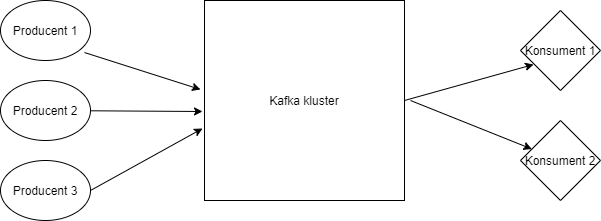
\includegraphics[scale=0.7]{img/prod-cons-model.png}
    \caption{Producent/konsument modellen med ett Kafka kluster.}
    \label{fig:mesh1}
\end{figure}

Datan som produceras av producenter i Kafka är \textit{händelser} (events). Händelserna har 3 olika
element: ett nyckelvärde, själva värdet av händelsen och en tidsstämpel. Till exempel, om vi har ett Kafka -kluster som intar telemetri från fartyg på havet så kan nyckelvärdet vara ett unikt nummer som fartyget har i ett datasystem så att händelsen kan kopplas samman med information av fartyget, värdet är kursen av fartyget och tidsstämpeln tiden när fartyget har skickat händelsen.

Kafka ger också möjligheten att dela in händelser i olika kategorier som kallas \textit{ämnen} (topics). Konsumenterna prenumererar till olika ämnen och får händelser från prenumererade ämnen.

\section{MapReduce}

När vi har förmågan att inta data från en dataström behöver vi också ett sätt för att hantera, slå ihop och analysera datan som kommer in. En mycket använd model är MapReduce -modellen. MapReduce är en programmeringsmodell som kan bearbeta massiva mängder data på ett kluster av datorer \citep{dean2008mapreduce}. MapReduce baserar sig på två funktioner 
som är bekanta från funktionella programmerings paradigmen, \textit{map} och \textit{reduce}. Data splittras först i mindre bitar och bitarna ges till MapReduce \textit{arbetare} (workers) som körs på en annan maskin eller prosess från huvudprosessen. Varje arbetare
kan få en eller flera bitar av datan. Arbetarna kör först funktionen map på datan och sedan reduce.

\subsection{Map och Reduce funktionerna}

MapReduce modellens map funktion kan beskrivas som en funktion $f: A \rightarrow B$ var $A = (S, S)$ och $B = (S, K)$ var $K$ är typen av datan som returneras. Map funktionen kan användas för till exemple filtrering,
transformering eller tolkning av serialiserad data. Funktionen returnerar en lista av tuplar som innehåller nyckeln och värdet. Map funktionen kans se ut till exempel såhär:

\begin{verbatim}
    def map(key: S, persons: S[]): (S, S)[] = {
      groupedByNameLength = persons.groupByNameLength()
      result = []
      for len in groupedByNameLength:
        append (len, 1) to result
      return result
    }
\end{verbatim}

MapReduce modellens reduce funktion tar in datan som returneras från map funktionen och slår ihop datan. 

\begin{verbatim}
    def reduce(keyFromMap: S, valueFromMap: (Int, Int)[]): Integer = {
      result = 0
      for value in valueFromMap:
        result = result + value
      return result
    }
\end{verbatim}

\subsection{MapReduce prosessen}

Ett MapReduce program har 7 olika steg. Först splittrats inkommande datan till $N$ segment. Efter splittringen
görs det flera noder av MapReduce programmet var en nod fungerar som \textit{mästare} (master) och andra
som arbetare. Mästarnoden tilldelar arbetarna map eller reduce arbeten. Arbetarna som har som uppgift att utföra map arbeten
läser ett segment som mästarnoden har givit den, kör funktionen map och sparar tupellistan i en buffert i minnet.
Innehållet av buffertarna skrivs under jämna mellanrun till en fil och arbetaren signalerar mästarnoden var datan för en viss
tupel finns i MapReduce klustret. Mästarnoden informerar arbetaren med reduce uppgifter om platser var datan sparad från map skedet
befinner. Datan läses och sorteras sedan så att tuplar med samma nyckel är gruperade tillsammans. Arbetaren kör reduce funktionen på varje
unika nyckel som finns i matade datan. Varje arbetare med ett reduce arbete skriver ut resultatet till en fil.

\begin{figure}[h]
    \centering
    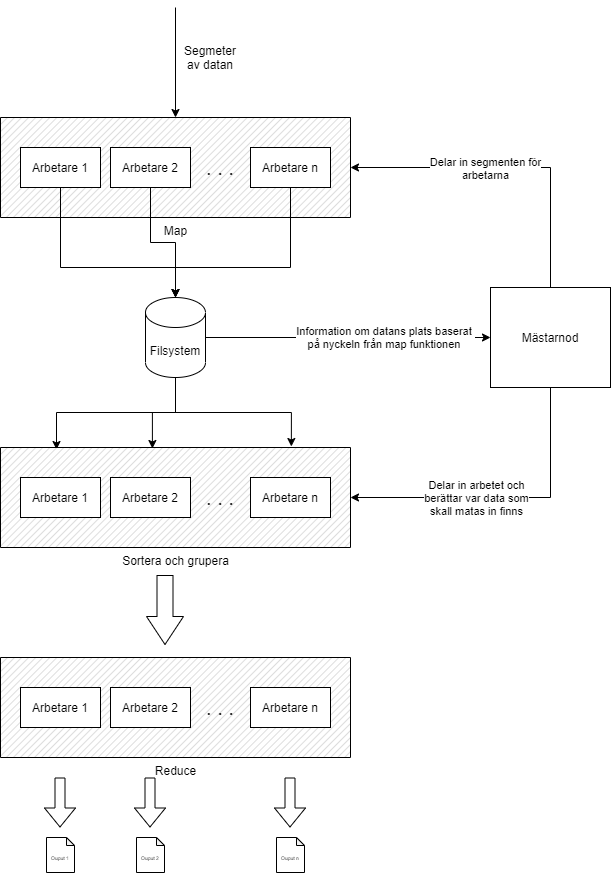
\includegraphics[scale=0.5]{img/map-reduce.png}
    \caption{MapReduce prosessen}
    \label{fig:mesh1}
\end{figure}

\section{Apache Storm}

Apache storm är ett distribuerat beräkningssystem \citep{apachestorm}. Apache Storm är gjort för att utföra arbeten
på samma sätt som i MapReduce, men göra dem i realtid och inte satsvist. Storm har några huvudkonsept: \textit{Topologier} (topologies),
\textit{strömmar} (streams), \textit{kranar} (spouts) och \textit{bultar} (bolts).
\begin{itemize}
    \item \textbf{Topologier} definierar hela strukturen av systemet. Topologier i Storm kan tänkas vara en graf av bultar och kranar.
    \item \textbf{Strömmar} är liknande till definitionen av dataströmmar som gavs tidigare. Strömmarna i Storm är sekvensser med tuplar som kan innehålla till exempel teckensekvenser eller heltal.
    \item \textbf{Kranar} i Storm är källan till en
eller flera strömmar. Kranar läser oftast data från en utomstående källa, till exempel ett Apache Kafka kluster, och avsänder dom till Storms topologi. Kranarna kan vara 
\textit{pålitliga} (reliable) var inkommande datan sparas och kan avsändas igen i fall något fel uppstår eller \textit{opålitliga} (unreliable)
var datan inte sparas.
   \item \textbf{Bultarna} sköter själva behandlingen av datan som kan vara i form av filtrering, sammanfattning, transformering 
eller sammanslagning. Bultarna prenumererar till en eller flera Storm strömmar varifrån bulten läser inkommande data. Färdiga datan från
bultarna kan skickas till en eller flera Storm strömmar.
\end{itemize}

Storm bultarna och kranarna körs på såkallade \textit{uppgifter} (tasks). Uppgifterna körs på egna trådar på en kluster av maskiner 
för att undvika blokering av andra uppgifter. Topologierna körs på en eller flera arbetar prosesser. Arbetar prosesserna kan till exempel vara
skillda prosesser på en maskin eller ett kluster av maskiner. En Storm grupering har 3 olika delar\citep{marz2013big}: Nimbus, Apache ZooKeeper 
kluster och Storm kluster. Nimbus är en mestarnod som ser till att topologin fungerar på rätt sätt och ger upfigter till arbetaren, ZooKeeper
används för at överse och orkestrera topologin och Storm klustret innehåller själva arbetarna. Varje nod med arbetare i storm klustret har en nod
som handleder andra arbetarnoderna. Handledaren tar kommandon från Nimbus och delegerar dem sedan framåt till arbetarnoderna.

Storm har ett system för pålitlighet som konstant granskar att tuplarna från strömmarna prosesseras i Storm topologin. Om en bult överskrider en
viss tidströskel under behandlingen så avbryts behandlingen av tupeln. Behandlingen av den obehandlade tupeln provas igen senare. 

\chapter{Behandlingsprosesser}

\section{Satsvis behandling av dataströmmar}

\textit{Satsvis behandling} (batch prosessing) av dataströmmar är en metod för behandling av 
dataströmmar som går ut på att köra behandlingsprogram på datan till exempel mellan jämna
tidsinterval eller när någon viss tröskel arr överskridit \citep{marz2013big}. Satsvisa behandligen
innehåller 3 olika steg. I först steget sparas inkommande datan. Nya inkommande datan kan sparas vart
som helst, men det är normalt at använda till exempel Apache Hadoops \textit{distribuerade 
filsystem} (Hadoop Distributed File System). Nya inkommande datan sparas i en skild plats från redan
mottagna datan (master data) för att hålla datan oföränderlig under nästa steget. I nästa steget prosesseras datan med till exempel
MapReduce som vi gick igenom i förra kapitlet. Före behandlingen påbörjas slås nya inkommande datan och gamla mottagna datan ihop.
Många olika MapReduce prosesser kan köras på datan och resultatet av en MapReduce prosess är oftast en vy av något som är
för komplicerat att producera i realtid. Datan från behandlingsskedet sparas oftast i en \textit{nyckel-värde} (key-value) databas som sedan kan användas
för att servera datan till olika applikationer.

\begin{figure}[h]
    \centering
    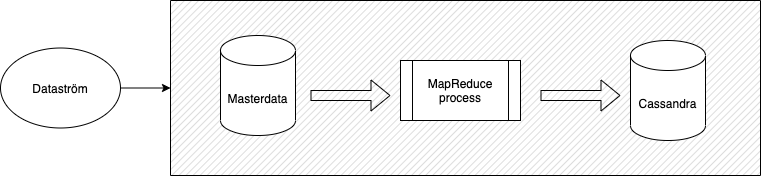
\includegraphics[scale=0.6]{img/batch-pipeline.png}
    \caption{En arkitektursbild av satsvis behandling av dataströmmar. Cassandra används som exempel av en nyckel-värde databas.}
    \label{fig:mesh1}
\end{figure}


\section{Behandling av dataströmmar i realtid}

I vissa fall är satsvisa behandlingen för långsam eftersom vyerna måst uppdateras genast när
nya händelser kommer in till systemet \citep{marz2013big}. I stället för att slå ihop gammal
data och ny data och köra en MapReduce prosess över all data för att uppdatera vyerna som i 
satsvis behandling, körs behandlingen bara på nya datan och nya vyn slås ihop med gamla vyn.
Eftersom datan kan komma in snabbare än vad det tar för systemet at prosessera inkommande datan
måste köar läggas till före behandlingssekeden för att undvika bortfallning av data. När datan
har kommit igenom kön behandlas den och slås ihop med förra vyn som systemet generera.

Användning av Apach Storm för behandling av dataströmmar i realtid är mycket normalt eftersom 
topologin av Storm tar hand om att varje händelse som intas blir prosesserad av systemet.

\begin{figure}[h]
    \centering
    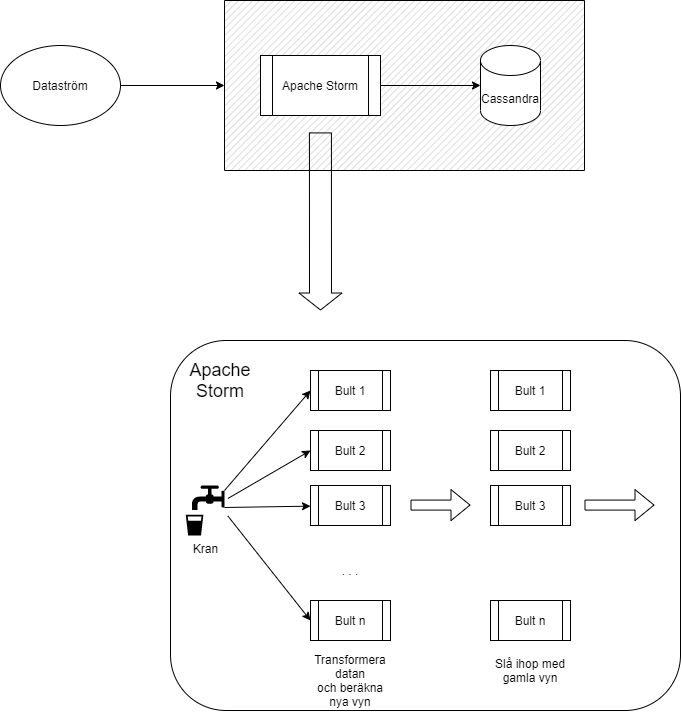
\includegraphics[scale=0.7]{img/speed-layer.png}
    \caption{Behandling av dataströmmar i realtid med Apache Storm. Cassandra som exempel av en nyckel-värde databas.}
    \label{fig:mesh1}
\end{figure}


\chapter{Arkitektur}

\section{Lambda arkitektur}

\section{Kappa arkitektur}

\section{Andra}

\chapter{Sammanfattning}
